\documentclass{standalone}

\ifstandalone
	\usepackage{amsmath}
	\usepackage{pgfplots}
\fi


\begin{document}
	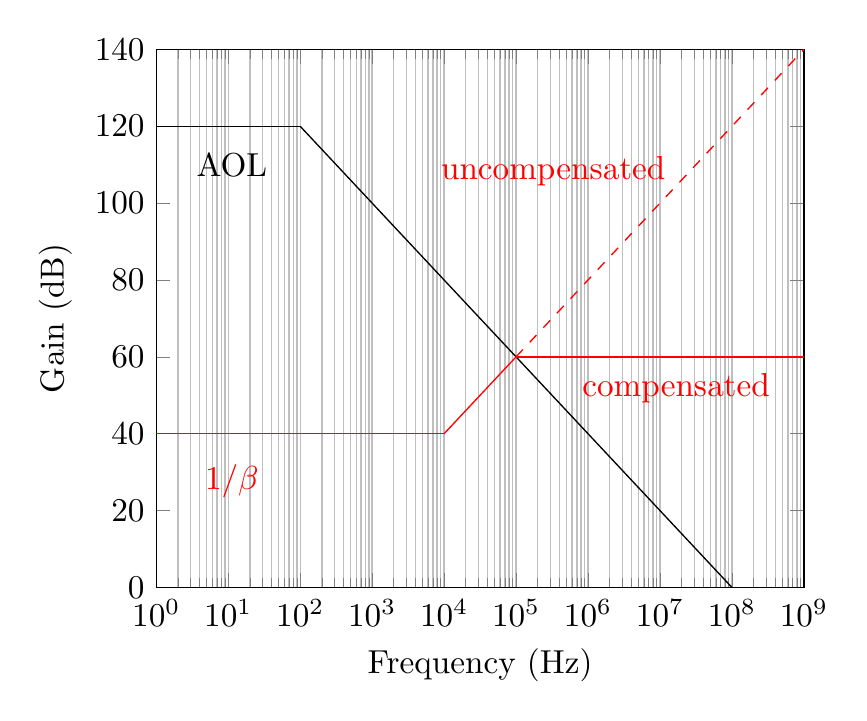
\begin{tikzpicture}[scale=1.2, transform shape]
		\begin{semilogxaxis}[xmin=1, xmax=1e9, xlabel=Frequency (Hz), ymin=0, ymax=140, ylabel=Gain (dB), ytick={0, 20, 40, 60, 80, 100, 120, 140}, grid=minor]
			\addplot[domain=1:1e2]{120};
			\addplot[domain=1e2:1e9]{160-20*log10(x)};
			\addplot[domain=1:1e4, color=red]{40};
			\addplot[domain=1e4:1e5, color=red]{-40+20*log10(x)};
			\addplot[domain=1e5:1e9, color=red]{60};
			\addplot[domain=1e5:1e9, dashed, color=red]{-40+20*log10(x)};
		\end{semilogxaxis}
		\node[label={AOL}] at (.8, 4.1) {};
		\node[label={[red]$1/\beta$}] at (.8, .7) {};
		\node[label={[red]compensated}] at (5.5, 1.7) {};
		\node[label={[red]uncompensated}] at (4.2, 4) {};
	\end{tikzpicture}
\end{document}
